\documentclass{article}
% PACKAGES
\usepackage[english]{babel}
\usepackage{graphicx} % Required for inserting images
\usepackage[most]{tcolorbox}
\usepackage{lmodern}
\usepackage{titlepic}
\usepackage{pdfpages}
\usepackage{tcolorbox}
\usepackage{tikz-cd}
\usepackage{amsmath}
\usepackage{multicol}
\usepackage{pgfplots}
\usepackage{xcolor}
\usepackage{tikz}
\usepackage{color,soul}
\usepackage{enumerate}
\usepackage{enumitem}
\usepackage{cancel}
\usepackage{hyperref} 
\usepackage{tikzsymbols}
\usepackage{fontawesome5}
\usepackage[export]{adjustbox}
\usepackage{amssymb}
\usepackage{tikz,lipsum,lmodern}
\usepackage{booktabs}


% COLOURS
\definecolor{Orchid}{RGB}{218, 112, 214}
\definecolor{snow}{rgb}{1.0, 0.98, 0.98}
\definecolor{mordantred19}{rgb}{0.68, 0.05, 0.0}
\definecolor{mistyrose}{rgb}{1.0, 0.89, 0.88}
\definecolor{nadeshikopink}{rgb}{0.96, 0.68, 0.78}
\definecolor{cadmiumgreen}{rgb}{0.0, 0.42, 0.24}
\definecolor{OliveGreen}{RGB}{85, 107, 47}
\definecolor{RoyalPurple}{RGB}{120, 81, 169}
\definecolor{NavyBlue}{RGB}{0, 0, 128}
\definecolor{CornflowerBlue}{RGB}{100, 149, 237}
\definecolor{Cerulean}{RGB}{0, 123, 167}
\definecolor{DarkOrchid}{RGB}{153, 50, 204}

\title{MCV4U - Calculus and Vectors [Chapter 6]}
\author{Kensukeken}
\date{April 30th, 2024}

\begin{document}
\maketitle

\tableofcontents
\newpage
\section{Unit 6}
\subsection{Introduction to Vectors}
A vector is a quantity that requires both a magnitude and a direction for a complete description.  Examples of vectors are weight, velocity and friction.  On the other hand, a scalar is a magnitude that can be completely specified by just one number.  Examples of scalars include age, volume, area, speed, mass and temperature.\\


A vector can be represented by a directed line segment.  The magnitude of the vector is indicated by the length of the line segment, and the direction of the vector is indicated by an arrowhead on the end of the segment.\\


Speed is a scalar quantity. We can describe the speed of an airplane as 200 km/h.\\


Velocity is a vector quantity. We can refer to the velocity of one airplane as $400 km/h$ in a southwesterly direction (represented by the vector $\vec{a}$ in the diagram) and the velocity of another airplane as 100 km/h in a northerly direction (represented by $\Vec{v}$)\\
\begin{figure}[h]
    \centering
    \includegraphics[width=0.9\textwidth]{imgs/a_v.png}
\end{figure}

We can indicate movement in a direction from one location to another using vectors. For example, the vector $\overrightarrow{AB}$ is a line segment running from A to B with its tail at A and its head at B. Its actual size, or magnitude, is denoted by $|\overrightarrow{AB}|$ , and is represented by the length of the line segment. The magnitude of a vector is always non-negative. The direction of the arrow represents the direction of the airplane, and its length represents the speed.
\newpage
\subsubsection{Equal Vectors}
\underline{Equal Vectors:}
Two vectors $\overrightarrow{AB}$ and $\overrightarrow{CD}$ are equal if and only if\\

\begin{enumerate}
    \item $\overrightarrow{AB}$ and $\overrightarrow{CD}$ are parallel to each other, and the direction from A to B is the same as the direction from A to B is the same as the direction from C to D.
    \item The magnitude of $\overrightarrow{AB}$ equals the magnitude of $\overrightarrow{CD}$. In other words, $|\overrightarrow{AB}|=|\overrightarrow{CD}|$
\end{enumerate}
\subsubsection{Opposite Vectors}
\underline{Opposite Vectors:}
Two vector $\overrightarrow{AB}$ and $\overrightarrow{CD}$ are opposite if and only if
\begin{enumerate}
    \item $\overrightarrow{AB}$ and $\overrightarrow{CD}$ are parallel to each other, and the direction from A to B is the opposite of the direction from C to D. Another way of putting this is that the direction from A to B is the same as the direction from D to C.
    \item The magnitude of $\overrightarrow{AB}$ equals the magnitude of $\overrightarrow{CD}$. In other words, $|\overrightarrow{AB}|=|\overrightarrow{CD}|$
\end{enumerate}
\subsubsection{Vector Addition}
\underline{Triangle Law of Addition}\\

You can determine the sum $\vec{a}+\vec{b}$ by putting the tail of $\vec{b}$ on the tip of $\vec{a}$ and then drawing a vector straight from the tail of $\vec{a}$ to the tip of $\vec{b}$. The resulting vector is called the resultant.

The method is sometimes also called the "tip to tail" method.
\begin{figure}[h]
    \centering
    \includegraphics[width=0.5\textwidth]{imgs/a+b.png}
\end{figure}


A way of thinking about the sum of two vectors is as follows:\\

If you start at Point A and walk to Point B, then walk from Point B to C, the net result is as if you walked from A directly to C.\\

Therefore, $\overrightarrow{AB}+\overrightarrow{BC}=\overrightarrow{AC}$.

\subsubsection*{Example}
Suppose that an airplane is travelling with a component velocity of 500 km/h N when it encounters a wind blowing with a velocity of 100 km/h E. What is resultant velocity?

\subsubsection*{Solution}
\begin{minipage}{0.45\textwidth}
    \centeringa
    \includegraphics[width=0.6\textwidth]{imgs/a_w_r.png}
\end{minipage}%
\begin{minipage}{0.4\textwidth}
    \begin{align*}
        |\vec{r}|^2 &= |\vec{a}|^2 + |\vec{w}|^2 \\
                    &= (500)^2 + (100)^2 \\
                    &= 200000 \\
        |\vec{r}| &\approx 509.9 \\
        \tan (\theta) &= \frac{100}{500} \\
        \theta &\approx 11.3^{\circ}
    \end{align*}
\end{minipage}
\vspace{2em}

    $\therefore$ The resultant velocity is approximately 509.9 km/h, N $11.3^{\circ}$

\subsubsection{Angle Between Two Vectors}
\hl{When you are told the angle between two vectors, it is always the angle between those vectors if they are drawn tail to tail.}
\\ \\ 
Note, however, that often when we add vectors, the angle that we use for our sine law or cos law calculations will not be that same value.
\subsubsection*{Example 2}
Two unit vectors $\vec{a}$ and $\vec{b}$ have an angle of $30^{\circ}$ between them. Determine the magnitude and direction of $2\vec{a}+\vec{b}$.
\subsubsection*{Solution}
We can start by drawing two diagrams:



\begin{figure}[h]
    \centering
    \includegraphics[width=0.7\textwidth]{imgs/a_b=30.png}
\end{figure}
\begin{minipage}{0.45\textwidth}
    \begin{align*}
        |\vec{r}|^2 &=|2\vec{a}|^2+|\vec{b}|^2-2|2\vec{a}||\vec{b}| \cos(150^\circ) \\
                    &=(2)^2+(1)^2-2(2)(1)\left(-\frac{\sqrt{3}}{2}\right) \\
                    &=5+3\sqrt{3} \\
        |\vec{r}|&\approx 2.91
    \end{align*}
\end{minipage}
\begin{minipage}{0.45\textwidth}
    \begin{align*}
        \frac{\sin \theta}{|\vec{b}|} &= \frac{\sin 150^\circ}{|\vec{r}|} \\
        \sin \theta &= 0.1718 \\
        \theta &= 9.9^\circ
    \end{align*}
\end{minipage}
\vspace{2em}

$\therefore$ The resultant vector has a magnitude of approximately 2.91 with a direction of approximately \textcolor{red}{$9.9^{\circ}$ rotated from $\vec{a}$ towards $\Vec{b}$}

\subsubsection*{Example}
In the picture below of a rectangle prism, we know that $$\overrightarrow{AB}= \vec{a}, \overrightarrow{AC}=\vec{b}, \overrightarrow{AE}=\vec{c}.$$\\
Determine an expression in terms of $\vec{a}, \vec{b}$ and $\vec{c}$ equal to each of the following

\subsubsection*{Solution}

\begin{minipage}{0.45\textwidth}
    \centering
        \includegraphics[width=0.7\textwidth]{imgs/abcdefgh.png}
\end{minipage}%
\begin{minipage}{0.5\textwidth}
    \begin{enumerate}
        \item[a)] 
        \begin{align*}    
            \overrightarrow{CH} &= \overrightarrow{CG} + \overrightarrow{GH} \\
                                &= \vec{c} + \vec{a}
        \end{align*}
        \item[b)] 
        \begin{align*}
            \overrightarrow{FG} &= \overrightarrow{FE} + \overrightarrow{EG} \\
                                &= -\vec{a} + \vec{b}
        \end{align*}
        \item[c)] $\overrightarrow{CF} = \vec{a} - \vec{b} + \vec{c}$ 
    \end{enumerate}
\end{minipage}

\subsubsection{Representing Vectors on a Cartesian Plane}
\textit{Components: }
We can repeat a two-dimensional vector on a Cartesian plane.

For example:
\begin{itemize}
    \item A vector that moves 1 unit to the right and 2 units up could be represented by the vector $\overrightarrow{(1,2)}$.
    \item A vector that moves 3 units to the left and 5 units down could be represented by the vector $\overrightarrow{(-3,-5)}$
    \item A vector that only moves 10 units down could be represented by the vector $\overrightarrow{(0,-10)}$
\end{itemize}
\subsubsection{Unit Vectors on the Cartesian Plane}\\


A unit vector is a vector with a magnitude of 1.\\

A vector that moves 1 unit to the right is $\overrightarrow{(1,0)}$ and a vector that moves 1 unit unit up is $\overrightarrow{(0,1)}$. These vectors are so significant that they are referred to as $\vec{i}$ and $\vec{j}$ respectively. In other words, $\vec{i}=\overrightarrow{(1,0)}$ and $\vec{j}=\overrightarrow{(0,1)}$.

All vectors represented with components on the two-dimensional Cartesian plane can be represented as a sum or difference of these unit vectors, for example,\\
$$\overrightarrow{(3,-4)}=3\overrightarrow{(1,0)}-4\overrightarrow{(0,1)}=3\vec{i}-4\vec{j}$$

\subsubsection{Distributive Property With Vectors}
\\

\textit{Component Form}
\subsubsection*{Example}
Simplify $3(2\vec{a}-5\vec{b}+\vec{c})-2(\vec{a}-4\vec{b}+6\vec{c})$
\subsubsection*{Solution}
\begin{align*}
    &=6\vec{a}-15\vec{b}+3\vec{c}-2\vec{a}+8\vec{b}-12\vec{c}\\
    &=4\vec{a}-7\vec{b}-9\vec{c}
\end{align*}
\subsubsection*{Example}
Given that $\vec{u}=(3,-1), \vec{v}=(-4,-7), \vec{w}=(10,1)$, state the components of the vector $4\vec{u}+2\vec{u}-7\vec{w}$
\subsubsection*{Solution}
\begin{align*}
    4\vec{u}-2\vec{v}=7\vec{w}&=4\overrightarrow{(3,-1)}+2\overrightarrow{(-4,-7)}-7\overrightarrow{(10,1)}\\
    &=\overrightarrow{(12,-4)}+\overrightarrow{(-8,-14)}-\overrightarrow{(70,7)}\\
    &=\overrightarrow{(12-8-70,-4-14-7)}=\overrightarrow{(-66,-25)}
\end{align*}
\subsubsection{Taking Different Paths Questions }
Another type of question is the "taking different paths" question. For some questions, you have to try getting from one place to another in a variety of ways unit a solution to your problem presents itself.
%% Continue this part later


\subsection{Forces}
Generally speaking, force can be defined as that which changes, or tends to change, the state of rest, or uniform motion of a body.\\
The description of a force's magnitude, without also specifying its direction, has little practical value. Since force has a magnitude and direction, therefore \underline{force is a vector.}\\

Often, there are a number of forces working on an object. 

\begin{itemize}
    \item The resultant force is the single force that would produce exactly the        same effect as all of the forces acting together.
    \item \textbf{Equilibrium} is a state in which an object does not move (i.e., its net force is 0).
    \item The \textbf{equilibrant} of a number of forces is the single force that opposes the resultant of the forces; therefore when the equilibrant is applied to the object, the object is in a state of equilibrium.  The equilibrant is equal to the resultant times negative 1.
\end{itemize}
The \textbf{Newton} is the unit of measurement for force.  One Newton is equal to the amount of force necessary to cause a mass of one kg to accelerate at one metre per second squared.  In other $1N=1kg \times m/s^2$

\subsubsection*{Example}
Two children, James and Fred, are pushing on a rock. James pushes with a force of 80 N in an easterly direction and Fred pushes with a force of 60 N in the same direction.Determine the resultant and the equilibrant of these two forces.
\subsubsection*{Solution}
\[\begin{tikzcd}
	{} && {} &&&& {}
	\arrow[""{name=0, anchor=center, inner sep=0}, "60"{pos=0.7}, from=1-3, to=1-7]
	\arrow["80", from=1-3, to=0]
\end{tikzcd}\]
$\therefore$ the resultant force is 140N east\\
the equilaterat force is 140N west

\begin{itemize}
    \item Of course, forces acting on an object are not always collinear.  The manner that we determine the resultant force is to add the vectors representing each of the individual forces.  We can use numerous different methods to do this, including
    \item the triangle law of addition of vectors, or
    \item the parallelogram law of addition, or
    \item adding components
\end{itemize}
 The best way to approach the situation will often depend on the specific question, and it will be helpful for us to recall the sin law and the cos law.
 
 $$\frac{\sin A}{a}=\frac{\sin B}{b}=\frac{\sin C}{c} \quad or \quad \frac{a}{\sin A}=\frac{b}{\sin B}=\frac{c}{\sin C}$$\\

 $$c^2=a^2+b^2-2ab\cos C$$
 Of course, we need to remember that the angle between two vectors refers to “tail-to-tail”, but often in our calculations we use the angle between the tip and the tail, which is a different value.
 \subsubsection*{Example}
Two forces of 20N and 40N act at an angle of $30^{\circ}$ to each other.  Determine the resultant of these two forces.
\begin{figure}[h]
    \centering
    \includegraphics[width=0.7\textwidth]{imgs/force_1.png}
\end{figure}
\begin{align*}
    |r|^2&=20^2+40^2-2(20)(40)\cos 150 ^{\circ}\\
    |r|&\approx 58.2\\
    \frac{\sin 150^{\circ}}{58.2}&\approx \frac{\sin \theta}{40}\\
    \theta &\approx 20.1^{\circ}
\end{align*}
$\therefore$ the resultant force is approximately 58.2N in a direction of $20.1^{\circ}$ related from the 20N force to the 40N force.\\
\newpage 

\subsubsection{Equilibrium:} A group of forces is said to be in equilibrium when there is no movement.
\begin{figure}[h]
    \centering
    \includegraphics[width=0.7\textwidth]{imgs/equilibrium.png}
    \caption{Forces in equilibrium}
\end{figure}

As you may notice, when there are two forces in equilibrium, they are opposite vectors.\\
When there are more than two forces in equilibrium, they form a closed polygon.
\subsubsection*{Example}
Given that three forces of 2 N, 3N and 4N are in equilibrium, determine the angle between the two smallest forces?
\subsubsection*{Solution}
\begin{figure}[h]
    \centering
    \includegraphics[width=0.5\textwidth]{imgs/force_2.png}
\end{figure}
\begin{align*}
    4^2=2^2+3^2-2(2)(3)\cos \theta\\
    16=4+9-12\cos \theta\\
    \theta \approx 104.5^{\circ}
\end{align*}
$\therefore$ the angle between the two smallest is approximately $75.5^{\circ}$
\newpage 

\subsubsection{Component Vectors}\\
It is often convenient to break a vector down into one or more vectors that together comprise the original vector.  
\begin{itemize}
    \item In two dimensions, this is most commonly done by considering the horizontal and vertical components of a vector.  
    \item In three dimensions, this is most commonly done by considering the components along each of the three axes.
\end{itemize}

\begin{minipage}[h]{0.4\textwidth}
    Consider the vector $\vec{f}$ shown at the right.\\
    We can break $\vec{f}$ down into a horizontal and a vertical component vector.\\
\end{minipage}
\begin{minipage}[t]{0.3\textwidth}
    \begin{tikzpicture}
        % Draw the vector f
        \draw[->, thick] (0,0) -- (4,3) node[midway, above left] {$\vec{f}$};
        
        % Draw the horizontal component
        \draw[dashed, ->] (0,0) -- (4,0) node[midway, below] {$\vec{f}_x$};
        
        % Draw the vertical component
        \draw[dashed, ->] (4,0) -- (4,3) node[midway, right] {$\vec{f}_y$};

        % Draw the right angle symbol
        \draw (4,0) -- (4.3,0) -- (4.3,0.3) -- (4,0.3) -- cycle;
        
        % Add labels to the points
        \node at (0,0) [below left] {O};
        \node at (4,0) [below] {A};
        \node at (4,3) [above right] {B};
    \end{tikzpicture}
    \[
    |\overrightarrow{f_x}| = |\overrightarrow{f}| \cos \theta
    \]
    \[
    |\overrightarrow{f_y}| = |\overrightarrow{f}| \sin \theta
    \]
\end{minipage}


\subsubsection*{Example}
Kayla pulls on a rope attached to her sleigh with a force of 200N. If the rope makes an angle of 20º with the horizontal, determine:
\begin{enumerate}
    \item[a)] the force that pulls the sleigh forward
    \item[b)] the force that tends to lift the sleigh
\end{enumerate}

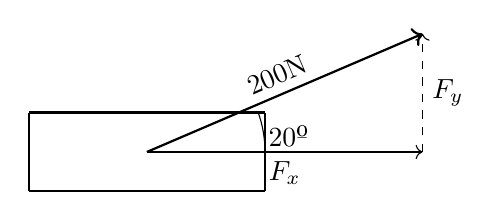
\begin{tikzpicture}
    % Draw the sleigh
    \draw[thick] (0,0) -- (3,0);
    \draw[thick] (3,0) -- (3,1);
    \draw[thick] (3,1) -- (0,1);
    \draw[thick] (0,1) -- (0,0);
    
    % Draw the rope
    \draw[thick,->] (1.5,0.5) -- (5,2) node[midway, above, sloped] {200N};
    
    % Draw the angle
    \draw[thick] (1.5,0.5) -- (5,0.5);
    \draw (3,0.5) arc (0:20:1.5);
    \node at (3.3,0.7) {20º};
    
    % Draw components
    \draw[dashed,->] (1.5,0.5) -- (5,0.5) node[midway, below] {$F_x$};
    \draw[dashed,->] (5,0.5) -- (5,2) node[midway, right] {$F_y$};
\end{tikzpicture}

\subsubsection*{Solution}

Let the force applied by Kayla be \( F = 200 \text{ N} \).

The force \( F \) can be decomposed into two components:
\begin{enumerate}
    \item[a)] The horizontal component (\( F_x \)) that pulls the sleigh forward.
    \item[b)] The vertical component (\( F_y \)) that tends to lift the sleigh.
\end{enumerate}

Using trigonometric identities:
\begin{itemize}
    \item \( F_x = F \cos(\theta) \)
    \item \( F_y = F \sin(\theta) \)
\end{itemize}

Given \( F = 200 \text{ N} \) and \( \theta = 20^\circ \):

\begin{enumerate}
    \item[a)] The force that pulls the sleigh forward:
    \[
    F_x = 200 \cos(20^\circ) \approx 200 \times 0.9397 = 187.94 \text{ N}
    \]
    \item[b)] The force that tends to lift the sleigh:
    \[
    F_y = 200 \sin(20^\circ) \approx 200 \times 0.3420 = 68.40 \text{ N}
    \]
\end{enumerate}

Therefore:
\begin{itemize}
    \item[a)] The force that pulls the sleigh forward is approximately \( 187.94 \text{ N} \).
    \item[b)] The force that tends to lift the sleigh is approximately \( 68.40 \text{ N} \).
\end{itemize}
\subsubsection*{Example}
A mass of 20 kg is suspended from a ceiling by two lengths of rope that make angles of 60º and 45º with the ceiling. Determine the magnitude of the tension in each rope.

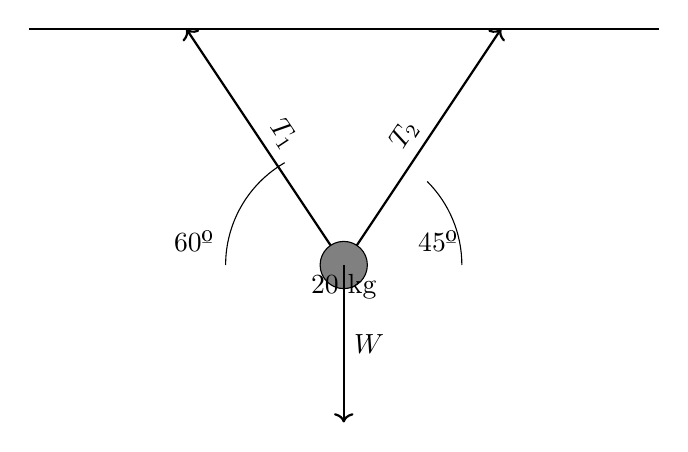
\begin{tikzpicture}
    % Draw the ceiling
    \draw[thick] (-4,3) -- (4,3);
    
    % Draw the ropes
    \draw[thick,->] (0,0) -- (-2,3) node[midway, sloped, above] {$T_1$};
    \draw[thick,->] (0,0) -- (2,3) node[midway, sloped, above] {$T_2$};
    
    % Draw the mass
    \draw[fill=gray] (0,0) circle (0.3) node[below] {20 kg};
    
    % Draw the angles
    \draw (1.5,0) arc (0:45:1.5);
    \node at (1.2,0.3) {45º};
    
    \draw (-1.5,0) arc (180:120:1.5);
    \node at (-1.9,0.3) {60º};
    
    % Draw weight
    \draw[thick,->] (0,0) -- (0,-2) node[midway, right] {$W$};
\end{tikzpicture}

\subsubsection*{Solution}

Given:
\[
W = mg = 20 \text{ kg} \times 9.8 \text{ m/s}^2 = 196 \text{ N}
\]

Using equilibrium conditions:
1. Horizontal equilibrium:
\[
T_1 \cos(60^\circ) = T_2 \cos(45^\circ)
\]
\[
T_1 \times 0.5 = T_2 \times 0.7071
\]
\[
T_1 = 1.4142 T_2
\]

2. Vertical equilibrium:
\[
T_1 \sin(60^\circ) + T_2 \sin(45^\circ) = W
\]
\[
T_1 \times 0.8660 + T_2 \times 0.7071 = 196
\]
\[
1.4142 T_2 \times 0.8660 + T_2 \times 0.7071 = 196
\]
\[
1.2247 T_2 + 0.7071 T_2 = 196
\]
\[
1.9318 T_2 = 196
\]
\[
T_2 = \frac{196}{1.9318} \approx 101.44 \text{ N}
\]

Now, substituting \( T_2 \) back into the equation for \( T_1 \):
\[
T_1 = 1.4142 \times 101.44 \approx 143.42 \text{ N}
\]

Therefore, the tensions in the ropes are:
\begin{itemize}
    \item \( T_1 \approx 143.42 \text{ N} \)
    \item \( T_2 \approx 101.44 \text{ N} \)
\end{itemize}
\subsection{Velocity}
\subsubsection*{Example 1}
A plane is heading due north with an air speed of 400 km/h when it is blown off course by a wind of 100 km/h from the northeast. Determine the resultant ground velocity of the airplane.

\begin{multicols}{2}
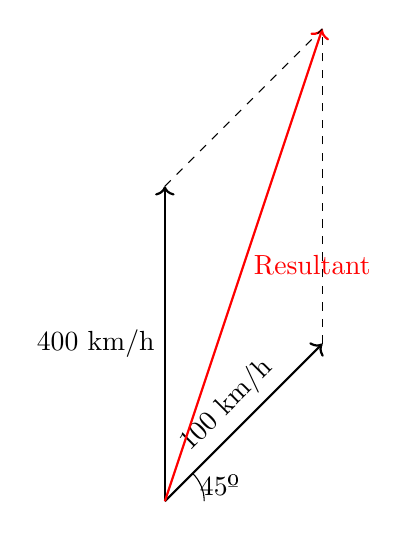
\begin{tikzpicture}
    % Plane velocity vector
    \draw[->, thick] (0,0) -- (0,4) node[midway, left] {400 km/h};
    
    % Wind velocity vector
    \draw[->, thick] (0,0) -- (2,2) node[midway, above, sloped] {100 km/h};
    
    % Resultant velocity vector
    \draw[->, thick, red] (0,0) -- (2,6) node[midway, right] {Resultant};
    
    % Components
    \draw[dashed] (0,4) -- (2,6);
    \draw[dashed] (2,2) -- (2,6);
    
    % Angle
    \draw (0.5,0) arc (0:45:0.5);
    \node at (0.7,0.2) {45º};
\end{tikzpicture}

\columnbreak

\subsubsection*{Solution}
\begin{align*}
    |\vec{r}|^2&=(400)^2+(100)^2-2(400)(100)\cos 45\\
    |\vec{r}|&\approx 336.8\\
    \frac{\sin \theta}{100}\approx \frac{\sin 45}{336.8}\\
    \theta &\approx 12.1^{\circ}
\end{align*}
$\therefore$ the resultant velocity is approx $336.8 km/h N 12.1^{\circ}w$

\end{multicols}

\subsubsection*{Example 2}
A plane is traveling 400 km/h in the direction W 25°N when it encounters a wind. As a result of the wind, the resultant velocity of the plane is 410 km/h, W 10°N. What is the velocity of the wind?

\begin{multicols}{2}
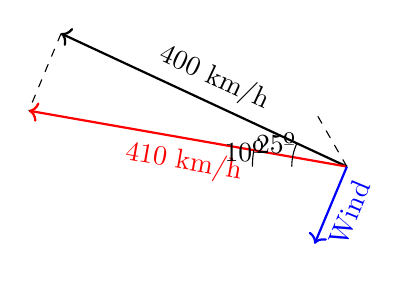
\begin{tikzpicture}
    % Plane initial velocity vector
    \draw[->, thick] (0,0) -- (-3.63,1.69) node[midway, above, sloped] {400 km/h};
    
    % Resultant velocity vector
    \draw[->, thick, red] (0,0) -- (-4.04,0.71) node[midway, below, sloped] {410 km/h};
    
    % Wind velocity vector
    \draw[->, thick, blue] (0,0) -- (-0.41,-0.98) node[midway, below, sloped] {Wind};
    
    % Components
    \draw[dashed] (-3.63,1.69) -- (-4.04,0.71);
    \draw[dashed] (0,0) -- (-0.41,0.71);
    
    % Angles
    \draw (-0.7,0) arc (180:155:0.7);
    \node at (-0.9,0.3) {25º};
    
    \draw (-1.2,0) arc (180:170:1.2);
    \node at (-1.3,0.2) {10º};
\end{tikzpicture}

\columnbreak

\subsubsection*{Solution}
\begin{align*}
    |\vec{w}|&=(410)^2(400)^2-2(410)(400)\cos 15\\
    |\vec{w}|&\approx 106.2\\
    (410)^2&=(400)^2+(106.2)^2-2(400)(106.2)\cos \theta\\
    \theta &\approx 87.9^{\circ}
\end{align*}
$\theta$ to the left of south is $\approx$ $22.9^{\circ}$\\
$\therefore$ the velocity of the wind is approx $106.2 km/h, s, 22.1^{\circ}$


\end{multicols}

\subsubsection*{Example 3}
A river is 2 km wide and flows at 6 km/h. Anna is driving a motorboat, which has a speed of 20 km/h in still water, and she heads out from one bank in a direction perpendicular to the current. A marina lies directly across the river from the starting point on the opposite bank.

\begin{multicols}{2}
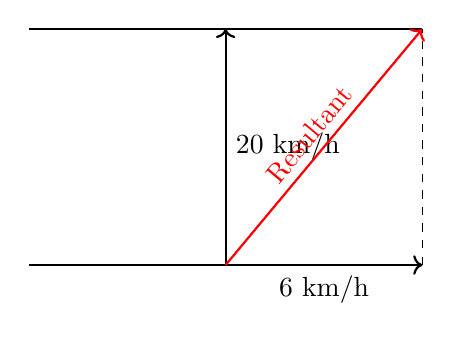
\begin{tikzpicture}
    % River banks
    \draw[thick] (0,0) -- (5,0);
    \draw[thick] (0,3) -- (5,3);
    
    % Boat velocity vector
    \draw[->, thick] (2.5,0) -- (2.5,3) node[midway, right] {20 km/h};
    
    % Current velocity vector
    \draw[->, thick] (2.5,0) -- (5,0) node[midway, below] {6 km/h};
    
    % Resultant velocity vector
    \draw[->, thick, red] (2.5,0) -- (5,3) node[midway, above, sloped] {Resultant};
    
    % Components
    \draw[dashed] (5,0) -- (5,3);
\end{tikzpicture}

\columnbreak

\subsubsection*{Solution}
\begin{itemize}
    \item a) Time to cross: \( \frac{2 \text{ km}}{20 \text{ km/h}} = 0.1 \text{ h} \) or 6 minutes.
    \item b) Distance downstream: \( 6 \text{ km/h} \times 0.1 \text{ h} = 0.6 \text{ km} \)
    \item c) To end up at the marina:
        \[
        \theta = \tan^{-1} \left( \frac{6}{20} \right) \approx 16.7^\circ \text{ upstream}
        \]
        Resultant velocity:
        \[
        V_{\text{resultant}} = \sqrt{(20 \cos(16.7^\circ))^2 + (20 \sin(16.7^\circ) - 6)^2} 
        \]
        \[
        \approx 19.2 \text{ km/h}
        \]
\end{itemize}

\end{multicols}
\end{document}
